\documentclass{article}
\usepackage{tikz}
\usetikzlibrary{arrows.meta, positioning}

\begin{document}

\begin{center}
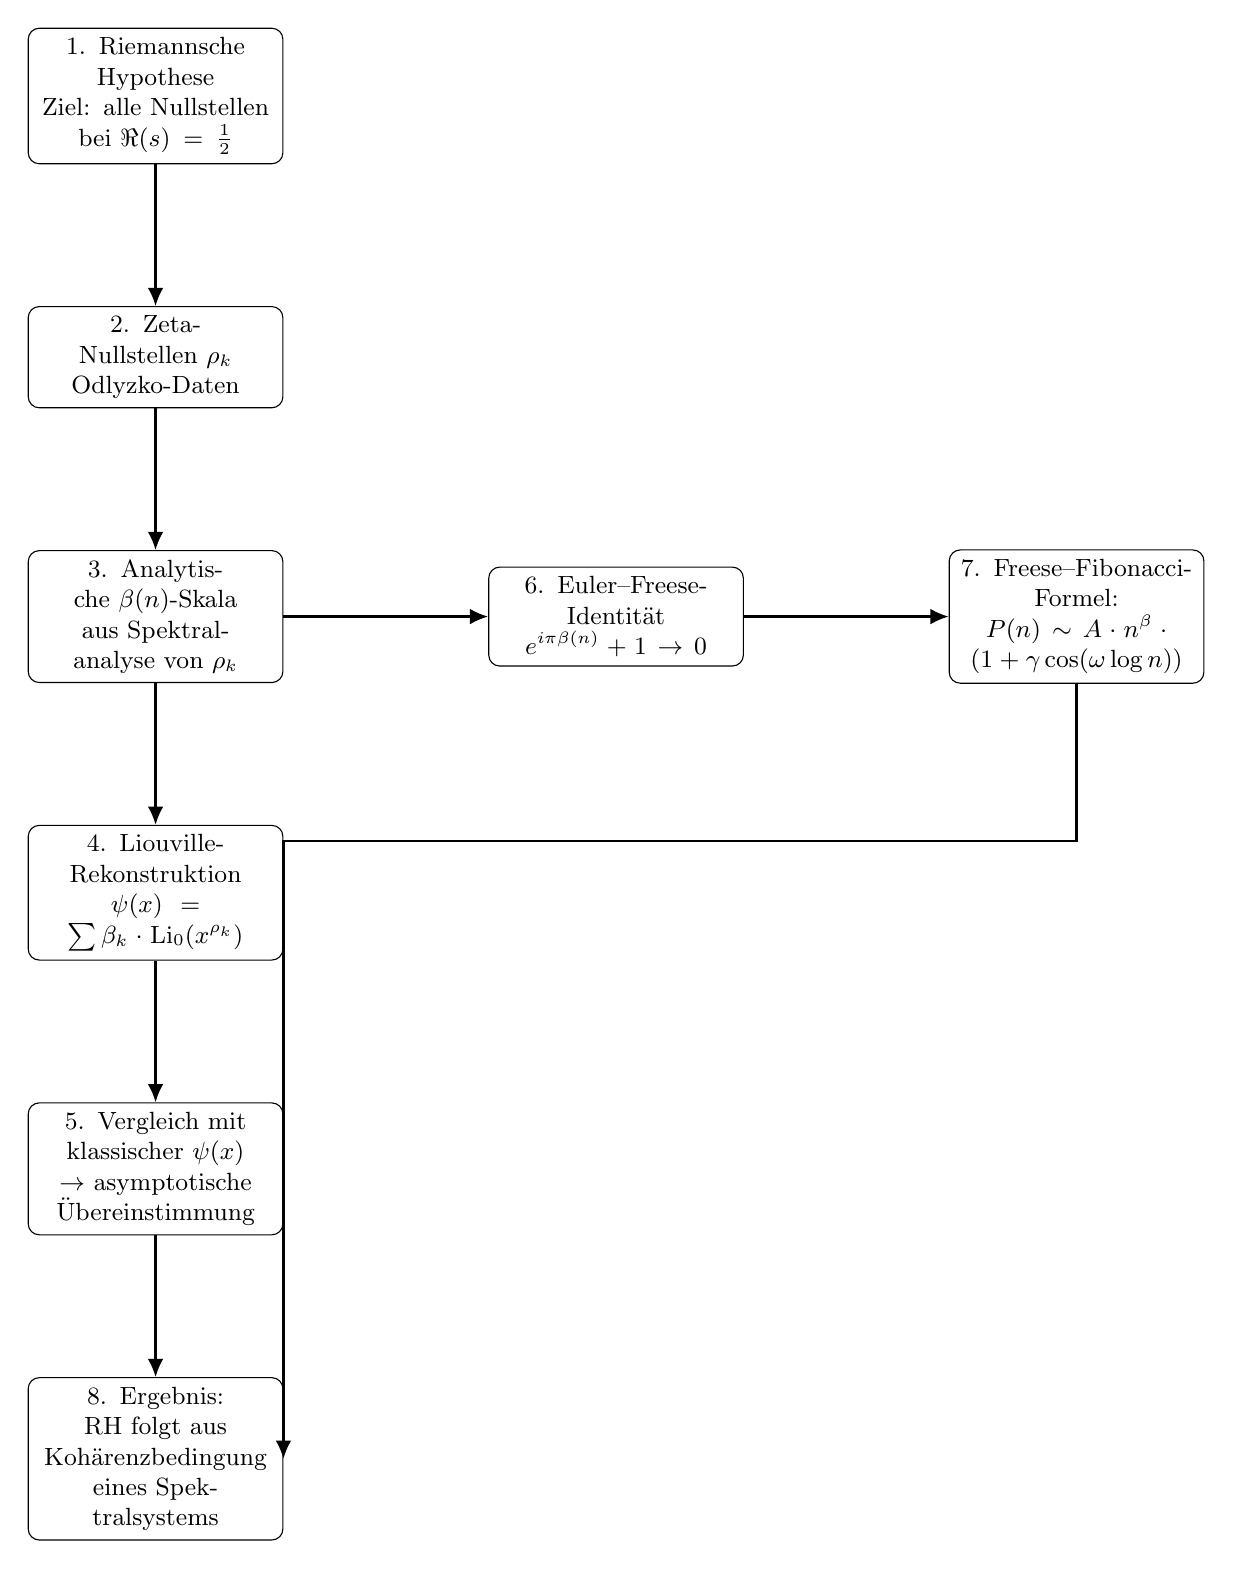
\begin{tikzpicture}[
  node distance=1.8cm and 2.6cm,
  every node/.style={align=center, font=\small},
  box/.style={draw, rectangle, rounded corners, text width=3cm, minimum height=1.2cm},
  arrow/.style={-{Latex[width=2mm]}, thick}
]

% Nodes
\node[box] (rh) {1. Riemannsche Hypothese\\Ziel: alle Nullstellen bei \(\Re(s) = \frac{1}{2}\)};
\node[box, below=of rh] (zeros) {2. Zeta-Nullstellen \(\rho_k\)\\Odlyzko-Daten};
\node[box, below=of zeros] (beta) {3. Analytische \(\beta(n)\)-Skala\\aus Spektralanalyse von \(\rho_k\)};
\node[box, right=of beta] (freese) {6. Euler–Freese-Identität\\\(e^{i\pi\beta(n)} + 1 \to 0\)};
\node[box, below=of beta] (liouville) {4. Liouville-Rekonstruktion\\\(\psi(x) = \sum \beta_k \cdot \mathrm{Li}_0(x^{\rho_k})\)};
\node[box, below=of liouville] (vergleich) {5. Vergleich mit klassischer \(\psi(x)\)\\\(\to\) asymptotische Übereinstimmung};
\node[box, below=of vergleich] (ergebnis) {8. Ergebnis:\\RH folgt aus Kohärenzbedingung\\eines Spektralsystems};
\node[box, right=of freese] (fib) {7. Freese–Fibonacci-Formel:\\\(P(n) \sim A\cdot n^\beta \cdot (1 + \gamma \cos(\omega\log n))\)};

% Arrows
\draw[arrow] (rh) -- (zeros);
\draw[arrow] (zeros) -- (beta);
\draw[arrow] (beta) -- (liouville);
\draw[arrow] (liouville) -- (vergleich);
\draw[arrow] (vergleich) -- (ergebnis);
\draw[arrow] (beta) -- (freese);
\draw[arrow] (freese) -- (fib);
\draw[arrow] (fib.south) |- ++(0,-2) -| (ergebnis.east);

\end{tikzpicture}
\end{center}

\end{document}